\chapter{Design Description}

\section{Overview}
A Gain/Phase Analyzer is an instrument used to plot the frequency response of a
network or amplifier. This project is a small, portable gain/phase analyzer, which
is controlled by a PC via USB and can perform analysis from 1~kHz to 150~MHz.

\begin{figure}[H]
\centering
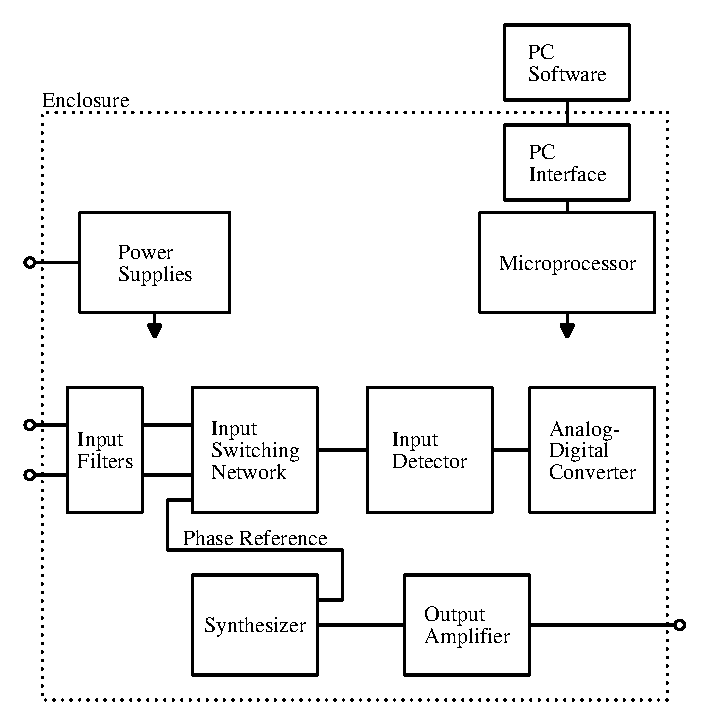
\includegraphics[width=5in]{systemdiagram}
\caption{System diagram}
\label{fig:sysdiag-dd}
\end{figure}

Gain/phase analyzers work by generating a sinusoidal stimulus signal, which is
applied to the device under test, and then measuring the signal that comes back
out of the device. This signal is generated by the Synthesizer, and feeds into
the Output Amplifier where it is boosted to an appropriate level for analysis.
After it returns from the devuce under test, it passes through input filtering
and protection, into a switch network. This allows one of two ports to be measured.
It is summed with a second signal from the synthesizer, which is used for phase
detection, and then passes to a logarithmic Detector which provides very sensitive
detection of the signal power level. The output of this detector is measured by an
Analog-Digital Converter that is under contrlo of a Microprocessor, and the data
is returned to the PC Software via the PC Interface.

\section{Detailed Description}

\subsection{Synthesizer}
This instrument needs to generate signals over a very wide range, from 1~kHz to
150~MHz (a range of over five orders of magnitude). To achieve this, a monolithic,
digital sinusoid synthesizer was used: the \texttt{AD9958} from Analog Devices.
This is a dual DDS (Direct Digital Synthesizer) operating at a sample rate of
500~MHz, with a pair 10-bit digital-analog converters~\cite{ad9958}.

This device generates differential current-mode outputs, which need to be
converted to a single-ended signal for transfer through the rest of the signal
path. A pair of wideband video amplifiers was used as differential amplifiers
with 0~dB gain to convert the signal.

\subsection{Output Signal Path}
Sometimes, it is necessary to decrease the output amplitude significantly, when
analyzing devices with high gain. The DDS features amplitude control, but this
is performed digtally, meaning that the digital resolution relative to the full-scale
signal amplitude decreases with the amplitude itself. This is acceptable only for
small variations. To facilitate larger shifts in amplitude, an analog, switchable,
15~dB attenuator comes next in the signal path. The M/A-COM \texttt{MAADSS0008} is
perfect for the application: a DC-coupled GaAs (gallium arsenide) switched 15~dB
attenuator with low insertion loss well past our bandwidth~\cite{maadss0008}. A
simple arrangement of discrete transistors level-shifts a control signal from the
microprocessor to provide the necessary negative bias to switch this.

After the attenuator, the signal passes through an antialiasing lowpass filter.
This is necessary because sampled systems inherently generate \emph{aliases},
or copies of the main signal that appear above the \emph{Nyquist rate}, which
in this case is at 250~MHz. These are undesirable as they could stimulate responses
in the device under test at frequencies we do not intend to measure. A seventh-order
elliptical filter provides a very sharp cutoff at approximately 150~MHz to remove
these from the signal.

The clean signal can now be amplified to drive the output. To achieve the specified
1.25~V~RMS output level, 30~dB of gain is required, which is difficult because of
the high bandwidth. This translates to a gain-bandwidth product of about 3.2~GHz
and a maximum slew rate of 1110~V/\us. A chain of two very advanced, high speed
operational amplifiers was used, at 15~dB each. The first is an Analog Devices
\texttt{AD8000}, which offers 1.5~GHz bandwidth and up to 4100~V/\us{} slew
rate~\cite{ad8000}. This amplifier is not sufficient to be the \emph{final} output amplifier,
though, as it cannot operate at a high enough voltage and does not have sufficient
slew rate under our operating conditions. The second amplifiers is a Texas Instruments
\texttt{THS3001}, which provides a lower 420~MHz bandwidth but an extremely high
6500~V/\us slew rate and can operate on supplies up to \Pos 16~V and \Neg 16~V~\cite{ths3001}.

\subsection{Input Signal Path}
Two input connectors are provided, to allow relative measurements from the input to the
output of a filter. The two input signals first pass through a small input protection
network. This is not hugely significant, as anything that is would risk affecting
the measurements. A pair of TVS diodes per input clamp off excessively large signals,
with a small series resistor providing an impedance for them to clamp against. This
provides enough power handling to quickly clamp off inputs from resonant devices under
test, but the user will have to exercise care if testing powered devices like amplifiers.

After the protection networks, the signal enters a pair of switches. These are
DC-coupled, GaAs switches with 2~GHz bandwidth, very similar to the attenuators
used in the output path~\cite{maswss0162}. An identical level-shifting circuit generates
the 0~V and \Neg 5~V bias voltages, and the two switches are connected with their
outputs in parallel and bias inputs interchanged to form a double-throw configuration.

The selected signal is buffered to prevent further circuitry from affecting the device
under test, which could interfere with measurements. A discrete buffer made from a very
high bandwidth (9~GHz) bipolar transistor is used --- the `excessively' high bandwidth
comes with an extremely low input capacitance, allowing the signal to be applied with a
purely resistive termination and no reactive impedance matching.

A phase reference signal (see \autoref{sub:phase}) is summed with the signal coming out
of the buffer, and the sum passes through a simple low-pass filter (fifth-order
Butterworth). This provides two functions. First, it removes external high-frequency
interference that may be picked up before the input connectors, and second, it removes
Nyquist aliases from the phase reference signal.

After the filter, the signal enters a logarithmic detector. This device provides an
output signal corresponding to the input power in decibels (nominally, 24~mV/dB~\cite{ad8310}),
which can be filtered down to a much lower frequency range and directly sampled by
an analog-to-digital converter.

\subsection{Phase Measurement}
\label{sub:phase}

Phase detection is not as simple to implement as amplitude detection. There are many
ways to do it, some of which are only realistically implemented for signals of known
amplitude.

The method used by this device is a null-finding approach. A second test signal (called
the ``phase reference''), of
identical frequency to the primary test signal and variable phase, is summed with the
input signal. The software steps the phase offset of this signal over the range from
0\dg{} to 360\dg, and tests the amplitude at each point. When the input signal to the
instrument and this phase reference are exactly 180\dg{} apart, they should interfere
destructively, summing to zero. The software performs a null search, testing for the
phase offset that produces this zero signal. To allow a high-precision search but
minimize the number of points tested, a recursive search is used: the entire range
from 0\dg{} to 360\dg{} is tested with a relatively small number of points, and then
these points are used to select a narrower range to re-test. The algorithm stops when
the search range is narrower than the desired measurement precision.

\subsection{Microprocessor}

The microprocessor in the instrument has a fairly simple job. It provides a bridge
between the PC and the instrument, via USB, generates control signals to the various
circuits in the instrument, and contains the analog-digital converter that samples the
signal from the logarithmic detector. The Atmel SAM4S is a series of ARM Cortex-M4
processors with all the necessary peripherals, a generous 120~MHz clock speed, and
full JTAG debugging support~\cite{sam4s};
this was used to provide all of these functions, of which it is
directly capable.

To provide backups in case this device proved troublesome, two alternatives were
selected. The system is designed to allow the use of an alternate microcontroller,
an Atmel ATMEGA32U4, and also can be used with an external USB interface controller,
an FTDI FT230XS. Neither of these was necessary in the end.

A Micro-USB connector provides interface to the PC. Signals pass through a pair of
termination resistors and a low-capacitance TVS diode array, and then directly into
the microprocessor. Power passes through a ferrite choke and into an simple circuit
that provides both inrush current limiting and power switchover, so that the
microcontroller is powered when either USB or the external power pack is present.

\subsection{Analysis}

The function of the PC software is relatively simple. To analyze a device under
test, the instrument is configured for logarithmically spaced test frequencies
over the desired test range, and the reoprted amplitude is queried. Then, the
null-finding algorithm (\autoref{sub:phase}) is applied to find the phase information.

If desired, this frequency response can then be saved and used as a template for
normalization. In this case, the saved amplitude (in decibels) and phase are subtracted
from a second analysis, to compensate for the attenuation and phase shift of the
analyzer itself and any test setup.

\section{Use}
The purpose of this device is provide students with tangible data when analyzing
circuits. As shown in \autoref{fig:contextdiag}, the device is to be connected between
a PC and a device under test; the user can initiate an analysis using the supplied software.
